% Yeban User Guide — Chapter 8: Export and Sharing (English)
% T-DOC-001 chapter-by-chapter delivery, written ahead of the CH08 task.
% Sources: app.slint export-dialog properties, docs/manual/06-export.md,
% export_stems.rs (stem receipt and manifest), README.md (CLI entry).

\chapter{Export and Sharing}
\label{ch:export-sharing}

\begin{quote}
既以为人己愈有，既以与人己愈多。
\end{quote}

Source: Laozi, Dao De Jing, ch. 81 (《道德经·第八十一章》). Translation: “The more one gives to others, the more one has; the more one shares, the more one gains.”

Export and sharing hand the work to others; the more you share, the more you gain.

Once a piece is finished it needs to leave Yeban: for mixing elsewhere, for mastering,
or simply as a playable file. This chapter covers what each export route produces and
how to verify the result — the word "complete" alone does not mean it exported right.

\section{WAV Export}

\subsection{Export the full mix}

File $\to$ Export Audio (WAV)... mixes the whole piece into one WAV file. The dialog
offers:

\begin{itemize}
  \item \textbf{Output path}: browse with Ctrl+O.
  \item \textbf{Sample rate}: can be specified; defaults to the project's (shown as \texttt{auto}).
  \item \textbf{Bit depth}: 24 by default.
  \item \textbf{Duration}: in seconds.
  \item \textbf{Bus limiter}: off by default; when on, rendering applies peak limiting on the bus to prevent clipping.
\end{itemize}

\screenshot{ch08-export-wav-dialog}{The Export Audio (WAV) dialog labelling path, sample rate, bit depth, duration and limiter toggle}

\subsection{Read the export receipt}

The export receipt gives measured readings: frame count, true peak and the limiter's
workload, plus the output location. These numbers come from the actual render, not
from copying back the input fields; whether the limiter was on and whether clipping
occurred should be read from the receipt, not guessed.

\section{Stem Export}

\subsection{When to use stems}

File $\to$ Export Stems... renders each source-node track into its own WAV, for mixing
in another program or for mastering. The master bus produces no file but is named in
the skipped list — that is not a dropped track.

Export runs on a background thread so the interface stays responsive; when it finishes
the status message reports how many stems were written, how many skipped and where.
Each stem is a 32-bit Float WAV at the project's sample rate, with a numbered filename
prefix; a \texttt{stems-manifest.json} index in the output directory records each
file's track identity, name, byte count and hash.

\screenshot{ch08-stems-toast}{The stem-export completion message showing written count, skipped count and output directory}

\subsection{Check the receipt, not just "complete"}

The stem receipt starts with a \texttt{exported-stems:} summary line, followed by one
line per stem and per skipped track. Beyond the track-level "skipped" count, look at
the \textbf{audio-clip} dimension: rendered/skipped clip counts. If every audio clip in
a stem was skipped, the message should downgrade to a warning rather than still saying
merely ``stems complete''. When you see ``complete'', cross-checking the clip counts
in the receipt is a good habit.

\begin{figure}[htbp]
\centering
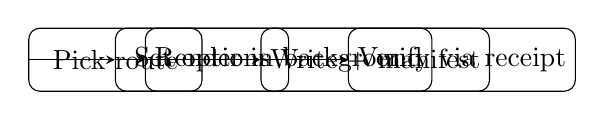
\begin{tikzpicture}[node distance=1.1cm, >=stealth,
    box/.style={draw, rounded corners, align=center, minimum width=2.2cm, minimum height=0.8cm}]
  \node[box] (a) {Pick route};
  \node[box, right of=a] (b) {Set options};
  \node[box, right of=b] (c) {Render in background};
  \node[box, right of=c] (d) {Write + manifest};
  \node[box, right of=d] (e) {Verify via receipt};
  \draw[->] (a)--(b); \draw[->] (b)--(c); \draw[->] (c)--(d); \draw[->] (d)--(e);
\end{tikzpicture}
\caption{Export flow: pick route $\to$ set options $\to$ render $\to$ write $\to$ verify with the receipt}
\label{fig:ch08-export-flow}
\end{figure}

The CLI can export stems too: \texttt{yeban-app --open X.yeban --export-stems stems/};
no window, no MCP session, and the same receipt convention as the GUI.

\section{Project Packaging and Archiving}

The \texttt{.yeban} file is itself the package: tracks, clips, notes, device chains and
the materials they use all live in one container, and saving is atomic (Chapter 2).
So "sharing a project" usually means handing over that file with the assets it
references; the asset pool is addressed by content hash, so opening it elsewhere does
not turn it silent.

Diagnostics $\to$ Export Project Diagnostic Bundle produces a troubleshooting bundle,
not artwork audio; attach it when asking someone to look at a broken project.

\section{Help Topic Mapping}

\begin{table}[htbp]
\centering
\caption{Sections of this chapter $\to$ in-app help anchors}
\label{tab:ch08-help}
\begin{tabular}{ll}
\hline
Section & Help topic \\
\hline
Full mix / dialog options & \texttt{export-wav-dialog} \\
Read the WAV receipt & \texttt{export-wav-receipt} \\
When to use stems & \texttt{export-stems-purpose} \\
Check the receipt, not just ``complete'' & \texttt{export-stems-receipt} \\
Project packaging and archiving & \texttt{export-project-archive} \\
\hline
\end{tabular}
\end{table}

\paragraph{What you will be able to do} Pick the right export route, set dialog options, verify output with the receipt (including clip counts), and know that a diagnostic bundle is not the piece.

\paragraph{Hands-on exercise} Export a full-mix WAV with the limiter on and read the frame count and true peak in the receipt; then export stems, check file names and byte counts against \texttt{stems-manifest.json}, and find the rendered/skipped audio-clip counts in the receipt; finally export stems for the same project from the CLI and compare the audio samples from both routes.
